\chapter{Available Results and Limitations}
\section{Result provenance}
Tables~\ref{tab:august} and \ref{tab:october} report archived output artifacts inspected during this preparation. Model inference and training were not rerun. August and October rows are distinct experiments with different splits and thresholds; they are not a controlled before/after comparison. Snapshot files and hashes are included under \texttt{evidence/}.

\begin{table}[htbp]
\centering\caption{August archived held-out results: 6,712 windows, including 1,575 FALL and 5,137 non-fall; the FP32 report identifies eight test subjects.}
\label{tab:august}
\begin{tabular}{@{}lrrr@{}}\toprule
Metric & FP32, $\tau=.5$ & FP32, $\tau=.3919$ & INT8, $\tau=.3919$\\\midrule
Sensitivity & .8235 & .8781 & .8743\\
Specificity & .8382 & .7818 & .7014\\
F1 & .7005 & .6781 & .6139\\
AUC-ROC & .9185 & .9185 & .8717\\\bottomrule
\end{tabular}
\end{table}
The corresponding quantization report records 18,904 bytes, input $[1,200,6]$, and output $[1,2]$. It records a 0.0804 absolute specificity reduction and a 0.0468 AUC reduction after quantization. Flash-budget compliance concerns the model file alone. No full-device memory or latency result follows from this table.

\begin{table}[htbp]
\centering\caption{October Colab log, archived FP32 evaluation. Total source windows: 38,426; reported train/validation/test counts: 31,714/3,005/3,707.}
\label{tab:october}
\begin{tabular}{@{}lrrr@{}}\toprule
Metric & Default .5 & Youden .5611 & Safety .4236\\\midrule
Sensitivity & .8057 & .7390 & .8981\\
Specificity & .8559 & .9146 & .7621\\
F1 & .7424 & .7560 & .7185\\
AUC-ROC & .9272 & .9272 & .9272\\\bottomrule
\end{tabular}
\end{table}
The October log records 126,856 augmented training windows and an 18,912-byte quantized export. The configuration instead lists a safety threshold of 0.4065 alongside the same safety metrics, while the log prints 0.4236. This disagreement blocks a settled deployed-threshold claim. The October INT8 export size is available; a matching held-out INT8 performance report is not established by the older August report. The 89.81\% safety sensitivity remains below the 90\% target.

The 38,426-window corpus count is an inventory, not the denominator of either held-out table. Neither retained report supplies a complete immutable list of held-out subject IDs. The name of a split helper does not establish class stratification; subject grouping and class balance must each be checked from the run manifest.

\section{Current verification and artifact inspection}
Current local array inspection confirms $(38426,200,6)$ float32 windows, 38 subject values, and 34 activity codes in the metadata. A byte comparison confirms that the firmware header contains the newer 18,912-byte model, not the August 18,904-byte file. These checks confirm shape and identity; they do not establish deployed inference.

The current Python suite passed 65 tests with 48 dependency warnings, and the repository structural verification passed four checks. Repository-wide Ruff verification failed on 23 pre-existing findings, and four files failed formatting checks. No unrelated code fixes or synchronization were performed as part of these reports. Software-test success does not validate actual I2C, physical BLE, battery life, or human evaluation.

\section{Historical laptop timings}
The tracker reports OpenVINO timing on an Intel Core Ultra 7 155H gateway over 5,000 inferences: CPU 0.131 ms, GPU 0.200 ms, and NPU 0.383 ms. These are \textbf{historical reported results}; the raw benchmark run and its complete warm-up/timing configuration were not reproduced here. They are not ESP32 latency, end-to-end detection delay, or power measurements.

\section{Power and feasibility estimates}
Operational endurance is governed by the effective battery capacity and the time-averaged subsystem current:
\begin{equation}
t = \frac{C_{\mathrm{eff}}}{I_{\mathrm{avg}}} = \frac{\eta_{\mathrm{usable}} \cdot C_{\mathrm{nom}}}{I_{\mathrm{avg}}}
\label{eq:battery_endurance}
\end{equation}
where $C_{\mathrm{nom}} = 1100\,\mathrm{mAh}$ denotes nominal cell capacity, $\eta_{\mathrm{usable}} \in [0.85, 0.95]$ represents usable discharge headroom before Low-Dropout (LDO) regulator dropout ($V_{\mathrm{cutoff}} \approx 3.3\,\mathrm{V}$), and $I_{\mathrm{avg}}$ is the average composite current.

Component current values are catalogued from official manufacturer datasheets in Table~\ref{tab:power_budget}.

\begin{table}[htbp]
\centering
\caption{Subsystem electrical current specifications from manufacturer datasheets.}
\label{tab:power_budget}
\small
\begin{tabular}{llrl}
\hline
\textbf{Subsystem} & \textbf{Operating Mode / Condition} & \textbf{Current ($I$)} & \textbf{Reference} \\
\hline
ESP32-S3 & Modem-sleep, 240\,MHz dual-core active & 49.6--64.1\,mA & \cite{espressif2024esp32s3}, Tab.~5-9 \\
ESP32-S3 & Modem-sleep, 240\,MHz SIMD (128-bit) vector load & 66.7--81.1\,mA & \cite{espressif2024esp32s3}, Tab.~5-9 \\
ESP32-S3 & Modem-sleep, 160\,MHz single/dual core active & 28.4--47.3\,mA & \cite{espressif2024esp32s3}, Tab.~5-9 \\
ESP32-S3 & Light-sleep ($V_{\mathrm{DD\_SPI}}$ \& RF gated) & 0.24\,mA & \cite{espressif2024esp32s3}, Tab.~5-10 \\
ESP32-S3 & Bluetooth LE RX active & 93.0\,mA & \cite{espressif2024esp32s3}, Tab.~5-8 \\
ESP32-S3 & Bluetooth LE TX active @ 0\,dBm (100\% duty) & 176.0\,mA & \cite{espressif2024esp32s3}, Tab.~5-8 \\
MPU-6050 & Gyroscope + Accelerometer normal operating & 3.8\,mA & \cite{invensense2013mpu6050}, \S6.3 \\
MPU-6050 & Accelerometer-only low power & 0.5\,mA & \cite{invensense2013mpu6050}, \S6.3 \\
MPU-6050 & Full-chip idle / sleep & 0.005\,mA & \cite{invensense2013mpu6050}, \S6.3 \\
Board Overhead & DevKit USB-UART bridge (CP2102) + LED & 10.0--15.0\,mA & Typical DevKit baseline \\
\hline
\end{tabular}
\end{table}

The widely cited estimate of $90\text{--}130\,\mathrm{mA}$ is derived from an \textbf{unoptimized development board baseline} operating without Dynamic Frequency Scaling (DFS) or modem sleep:
\begin{align}
I_{\mathrm{unoptimized}} &= I_{\mathrm{MCU,240MHz}} (50\text{--}65\,\mathrm{mA}) + I_{\mathrm{MPU}} (3.8\,\mathrm{mA}) + I_{\mathrm{BLE,avg}} (15\text{--}35\,\mathrm{mA}) + I_{\mathrm{board}} (10\text{--}15\,\mathrm{mA}) \nonumber \\
&\approx 80\text{--}118\,\mathrm{mA}
\end{align}
Peak transmission bursts and neural inference passes elevate transient demand to $\approx 130\,\mathrm{mA}$. Under nominal cell capacity ($C_{\mathrm{nom}} = 1100\,\mathrm{mAh}$, $\eta_{\mathrm{usable}} = 1.0$), this yields an idealized operating window of $t = 1100 / [90, 130] \approx 8.5\text{--}12.2\,\mathrm{hours}$ ($7.2\text{--}10.4\,\mathrm{hours}$ at $\eta_{\mathrm{usable}} = 0.85$).

Conversely, an \textbf{optimized production firmware baseline} (160\,MHz CPU, BLE slave connection latency, customized PCB omitting the USB bridge, and low-quiescent LDO $I_q < 50\,\mu\mathrm{A}$) projects:
\begin{equation}
I_{\mathrm{optimized}} \approx 30\,\mathrm{mA} (\mathrm{MCU}) + 3.8\,\mathrm{mA} (\mathrm{MPU}) + 3.0\,\mathrm{mA} (\mathrm{BLE}) + 0.1\,\mathrm{mA} (\mathrm{LDO}) \approx 37\,\mathrm{mA}
\end{equation}
which theoretically extends endurance to $t \approx 1100 / 37 \approx 29.7\,\mathrm{hours}$ ($25.2\,\mathrm{hours}$ at $\eta_{\mathrm{usable}} = 0.85$).

Both projections are analytical estimates derived from component datasheets. Actual operating battery life remains unmeasured until empirical current logging across all operational regimes is conducted on final assembled hardware. Older narratives citing 16--28 hours mixed unoptimized active draw with deep-sleep assumptions and are superseded by this derivation.

\section{Statistical and domain limitations}
Saved point estimates lack subject-clustered confidence intervals and complete immutable split manifests. Correlated windows are not independent volunteers. Future uncertainty analysis should resample at the subject or episode level, retaining paired predictions and reporting 95\% confidence intervals. For demographic cohorts with $n<30$, flag insufficient sample support and avoid subgroup rankings; the overall exploratory pilot must still report counts and limitations.

Event sensitivity, false alarms per hour, physical timing, wrist transfer, and elderly clinical performance remain unmeasured. Integrated evaluation must include every annotated fall, including gate rejections; classifier recall alone conceals gate misses.

\section{Kinematic Feature Attribution and Explainability Analysis}
Input-times-gradient attribution shows that the 1D CNN distributes its sensitivity across all six IMU axes with a modest $a_z$ lead, and it does not show temporal concentration within a fixed impact segment. Attributions $A_{t,c} = X_{t,c}\,\partial P(\mathrm{FALL})/\partial X_{t,c}$ were computed for 300 fall-labelled windows sampled (seed 42) from the 6{,}712-window subject-disjoint test split, and for up to 30 windows each of four high-acceleration ADL codes (Issue~\#12). Windows were sampled by label, not filtered by correct prediction. Per window, absolute attributions were summed over time and normalized to unit sum across channels. These are gradient saliency summaries, not Shapley values; the ``shap'' prefix in figure filenames is a legacy identifier.

\begin{figure}[htbp]
\centering
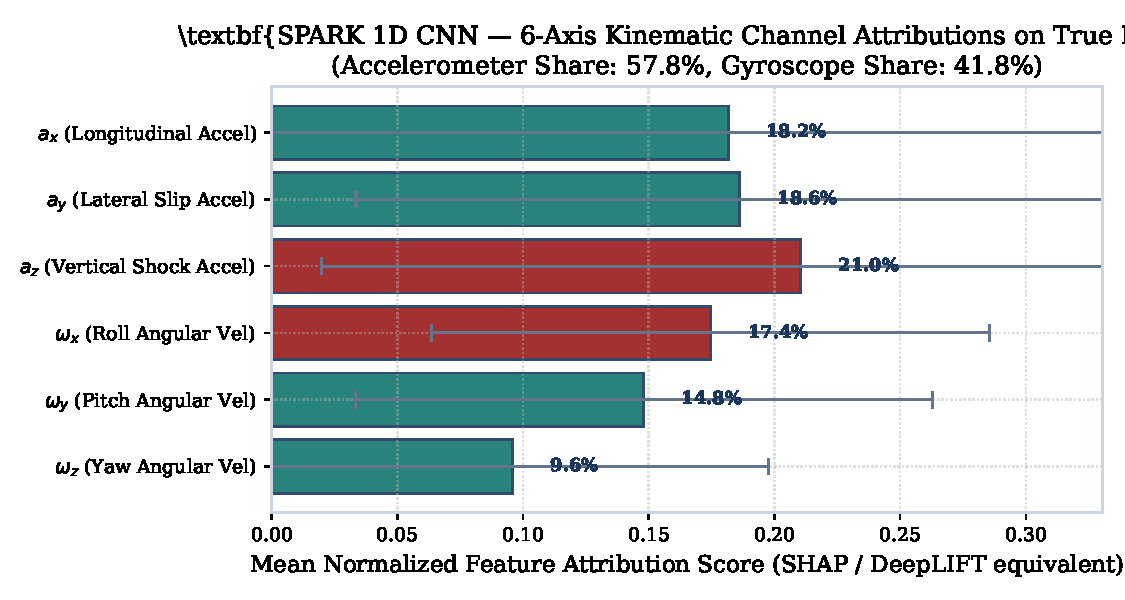
\includegraphics[width=0.88\textwidth]{Figures/fig_shap_channel_attribution.pdf}
\caption{Mean normalized channel attribution over 300 held-out fall-labelled windows. A uniform split would assign 16.7\% per channel; error bars (one standard deviation) overlap across most channels.}
\label{fig:shap_channel}
\end{figure}

Accelerometer channels receive $57.8\%$ of attribution and gyroscope channels $41.8\%$ (Figure~\ref{fig:shap_channel}). The largest single channel is $a_z$ ($21.0 \pm 19.1\%$), followed by $a_y$ ($18.6 \pm 15.3\%$), $a_x$ ($18.2 \pm 18.5\%$), and $\omega_x$ ($17.4 \pm 11.1\%$); $\omega_z$ is lowest ($9.6 \pm 10.2\%$). The leading channels sit within a few percentage points of the uniform $16.7\%$ and their per-window spread exceeds the gaps between them, so the ranking is not stable at the window level. The defensible reading is that the model uses all axes, with weaker reliance on yaw rate, rather than that it detects a specific vertical-impact signature. Axis labels are in the device frame; without a fixed wrist orientation they do not map to gravity-aligned ``vertical'' or ``lateral'' directions.

\begin{figure}[htbp]
\centering
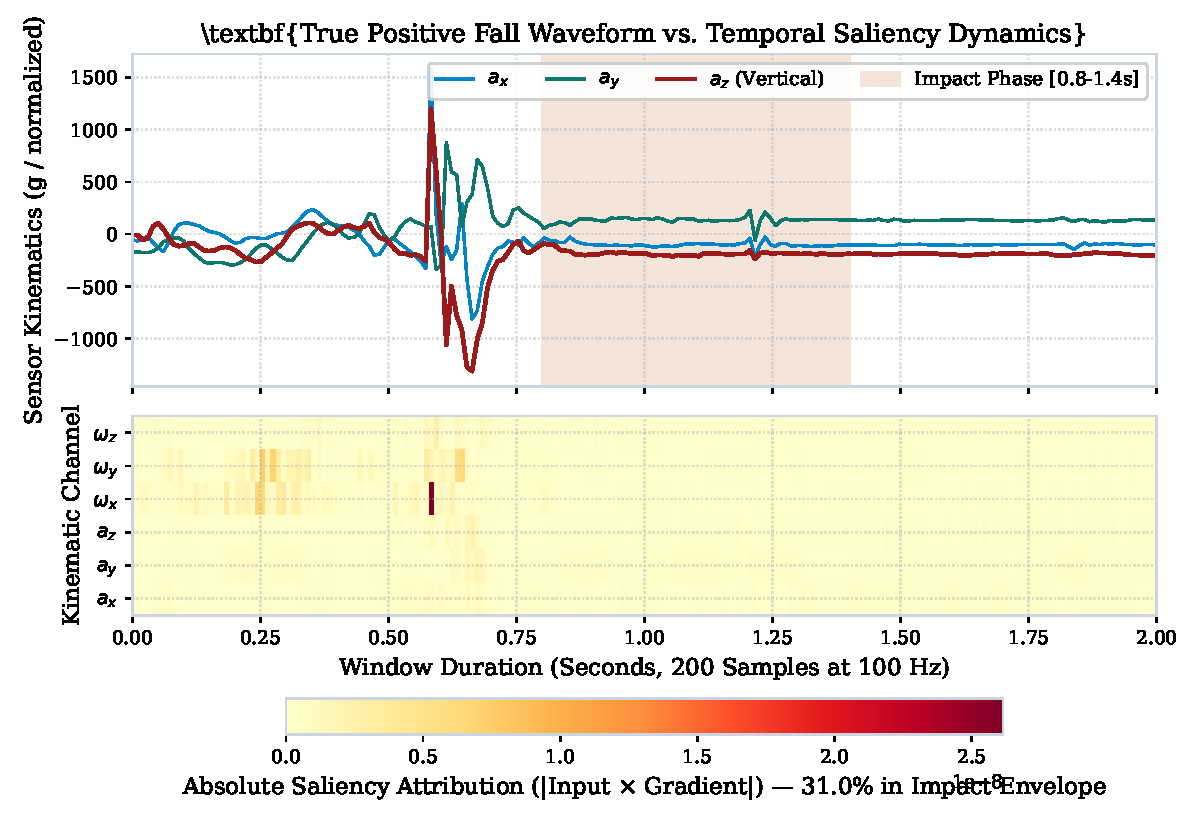
\includegraphics[width=0.88\textwidth]{Figures/fig_shap_temporal_saliency.pdf}
\caption{Signal and absolute attribution for the single highest-scoring sampled fall window (200 samples at 100\,Hz). The shaded band marks the fixed 0.8--1.4\,s segment, which is not aligned to an annotated impact; this example is illustrative and not representative of the cohort.}
\label{fig:shap_temporal}
\end{figure}

Across the 300 windows, the fixed segments receive $38.5\%$ (0.0--0.8\,s), $31.0\%$ (0.8--1.4\,s), and $30.1\%$ (1.4--2.0\,s) of attribution mass. These segments cover $40\%$, $30\%$, and $30\%$ of the samples, so attribution is distributed in proportion to duration and shows no concentration in the middle segment. Because falls are not aligned to a common impact time across windows, this null result does not show that the model ignores impact; it shows that fixed-segment averaging cannot test that claim. An impact-aligned analysis, re-centring each window on its peak acceleration magnitude, is required before any temporal claim is made.

\begin{figure}[htbp]
\centering
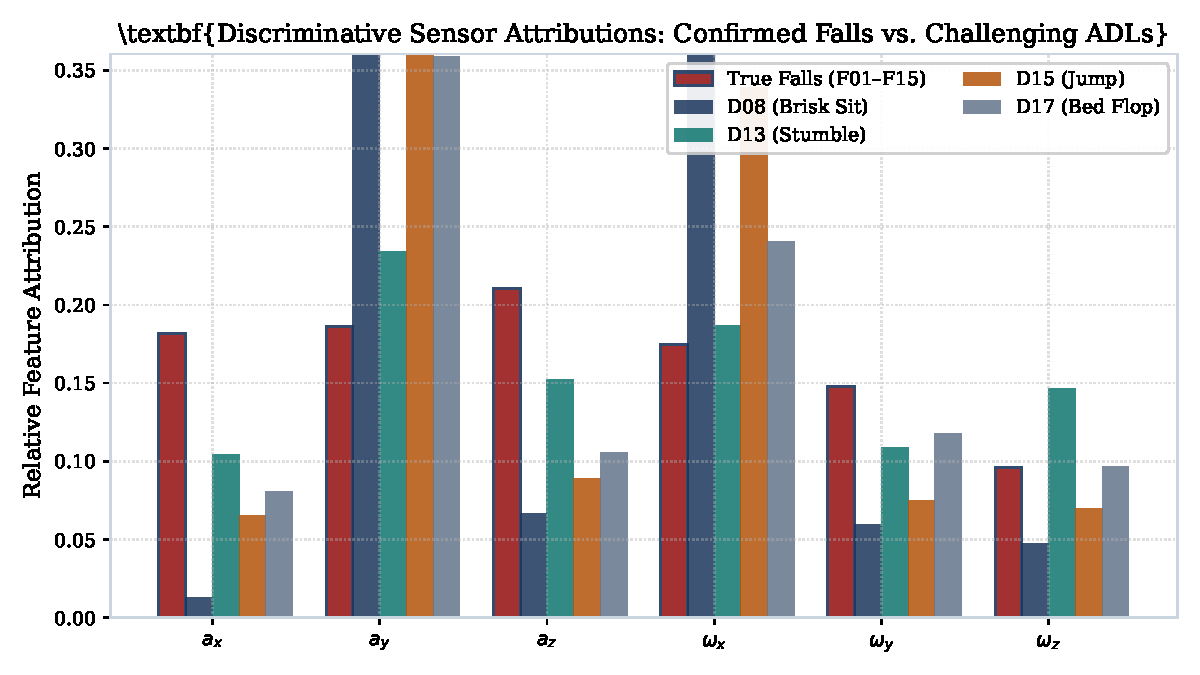
\includegraphics[width=0.88\textwidth]{Figures/fig_shap_fall_vs_adl_contrast.pdf}
\caption{Comparative feature attributions contrasting confirmed falls against challenging high-acceleration ADLs (D08 fast sit, D13 stumble, D15 jump, D17 bed flop).}
\label{fig:shap_adl_contrast}
\end{figure}

For the ADL groups (Figure~\ref{fig:shap_adl_contrast}), $a_z$ attribution is lower than for falls: $6.6\%$ (D08), $15.2\%$ (D13), $8.9\%$ (D15), and $10.6\%$ (D17). D08, D15, and D17 instead concentrate on $a_y$ ($36$--$43\%$) and $\omega_x$ ($24$--$38\%$), while D13 is spread more evenly. This shows that the gradient of $P(\mathrm{FALL})$ responds to different channels for these activities. It does not show how the classifier rejects them: attribution is reported for all sampled windows regardless of predicted class, group sizes are at most 30 windows drawn from few subjects, and no per-activity false-alarm rate is reported alongside. Linking attribution patterns to false-alarm behaviour requires the per-activity confusion counts and subject-level resampling described in the statistical limitations above.
